\documentclass{standalone}
\usepackage{tikz}
\usetikzlibrary{arrows.meta}
\definecolor{spring}{HTML}{586e75}
\definecolor{back}{HTML}{fdf6e3}

\begin{document}

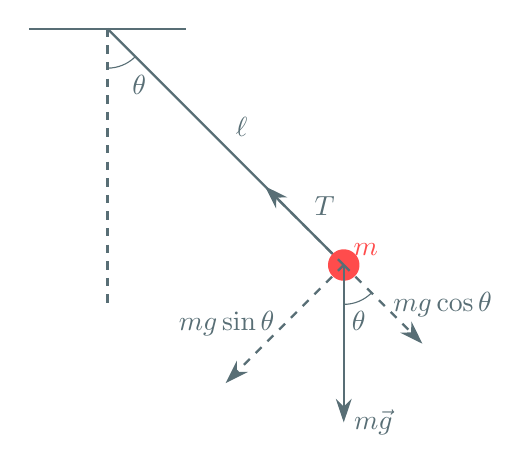
\begin{tikzpicture}
    % Draw the ceiling
    \draw[thick, spring] (-1,0) -- (1,0);

    % Draw the vertical line where the pendulum attaches to the ceiling
    \draw[thick, dashed, spring] (0,0) -- (0,-3.5);

    % Draw the pendulum rod
    \draw[thick, spring] (0,0) -- (3,-3) node[midway, above right] {$\ell$};

    % Draw the pendulum mass
    \fill[red!70] (3,-3) circle (0.2) node[above right] {$m$};

    % Draw the gravity force vector
    \draw[-{Stealth[length=3mm,width=2mm]}, thick, spring] (3,-3) -- (3,-5) node[right] at (3, -5) {$m\vec{g}$};

    % Decompose the gravity into central and perpendicular components
    \draw[-{Stealth[length=3mm,width=2mm]}, thick, dashed, spring] (3,-3) -- (1.5,-4.5) node[midway, left] {$mg \sin\theta$};
    \draw[-{Stealth[length=3mm,width=2mm]}, thick, dashed, spring] (3,-3) -- (4,-4) node[midway, right] {$mg \cos \theta$};
    \draw[-{Stealth[length=3mm,width=2mm]}, thick, dashed, spring] (3,-3) -- (2,-2) node[midway, above right] {$T$};

    % Draw the angle theta between the vertical line and the pendulum
    \draw[spring] (0,-0.5) arc (270:315:0.5) node[midway, below right, spring] {$\theta$};
    \draw[spring] (3,-3.5) arc (270:315:0.5) node[midway, below, spring] {$\theta$};

\end{tikzpicture}

\end{document}
